\documentclass{article}


\usepackage{arxiv}

\usepackage[utf8]{inputenc} % allow utf-8 input
\usepackage[T1]{fontenc}    % use 8-bit T1 fonts
\usepackage{hyperref}       % hyperlinks
\usepackage{url}            % simple URL typesetting
\usepackage{booktabs}       % professional-quality tables
\usepackage{nicefrac}       % compact symbols for 1/2, etc.
\usepackage{microtype}      % microtypography
\usepackage{fancyhdr}       % header
\usepackage{graphicx}       % graphics
\usepackage[table, x11names, svgnames]{xcolor}
\usepackage{subfig}
\usepackage{float}
\usepackage{caption}
\usepackage[section]{placeins}
\usepackage{setspace}
\usepackage{overpic}

\setstretch{1.2} % line spacing

\graphicspath{{assets/}}

%% Header
\pagestyle{fancy}
\thispagestyle{empty}
\rhead{ \textit{ }} 
\fancyhead[LO]{}

% \fancyhead[RE]{Firstauthor and Secondauthor} % Firstauthor et al. if more than 2 - must use \documentclass[twoside]{article}

%% Title
\title{Clinical advancement forecasting
%% Cite as
\thanks{\textit{\underline{Citation}}: 
\textbf{TBD}} 
}

%% Authors
\author{
  Authors TBD \\
  Related Sciences \\
%   %% examples of more authors
%    \And
%   Author3 \\
%   Affiliation \\
%   Univ \\
%   City\\
%   \texttt{email@email} \\
}

%% Body
\setlength{\parindent}{20pt}

\begin{document}
\maketitle

%% Variables
\def\evaluationDatasetPairCount{9010}
\def\topRankingPct{2}
\def\bottomRankingPct{98}

\begin{abstract}
Choosing which drug targets to pursue for a given disease is one of the most impactful decisions made in the global development of new medicines. This study examines the extent to which the outcomes of clinical trials can be predicted based on a small set of longitudinal (temporally labeled) evidence and properties of drug targets and diseases. We demonstrate a novel statistical learning framework utilizing both constrained and unconstrained linear and tree models, that can predict clinical advancement for the top \topRankingPct\% of target-disease pairs 1.5-2x more effectively than Open Targets composite scores as well as common measures of genetic support that have already been established -- and observed in this study -- to confer a 2x higher likelihood of success (a 3-4x cumulative improvement). Utilizing a subset of our biomedical evidence base, non-negative linear models can produce simple weighting schemes across various types of human, animal, and cell model genomic, transcriptomic, proteomic, and clinical evidence to identify target-disease pairs with high probabilities of advancing beyond phase 2 trials, and uncover a range of previously undeveloped target-disease pairs poised for clinical success. In this study we further explore: i) how longitudinal treatment of evidence relates to leakage and reverse causality in biomedical research and how temporalized evidence can mitigate common forms of potential biases and inflation ii) the relative impact of different type of features on our predictions; and iii) an analysis of the space of currently undeveloped, tractable targets predicted with these methods to have the highest likelihood of clinical success. To ease reproduction and deployment, no data is used outside of Open Targets and the described methods require no expert knowledge, and can support expansion of lines of evidence to further improve performance.
% Note: OT multipliers come from Sensitivity / Relative risk ratio distribution across configurations / mean@10 and mean@20
\end{abstract}

\section{Introduction}
\label{sec:introduction}

It has been well established that drugs with human genetic evidence linking their respective targets to indications in clinical trials are more likely to succeed \cite{Nelson2015-eg,King2019-rc,Minikel2023.06.23.23291765,Razuvayevskaya2023.02.07.23285407,PMID:30652614,PMID:24833294,PMID:35804044,PMID:37803084,PMID:36963162}, and to a lesser extent, that the same may also be true for single-cell transcriptomic evidence \cite{Dann2024.04.04.24305313}. This information has been used to devise target and target-disease ranking algorithms based primarily on a synthesis of multiple genetic signals alone \cite{PMID:38172303,Koscielny2017-rr,PMID:31253980}. It is also possible to expand the breadth of this genetic support to more targets and diseases based on knowledge graphs, protein interactions and/or disease ontologies \cite{PMID:33262371,Bao2022-bq,Sadler2023-xd,PMID:36087372,PMID:36823319}. To our knowledge, all such expansion methods identify a larger space of opportunities at the expense of expected success rates. This is not a focus of this work as we aim, instead, to establish a framework for identifying target-disease (TD) pairs with the very highest possible likelihood of success. We accomplish this by integrating human clinical, genetic/genomic, transcriptomic and proteomic data as well as cell/animal model evidence, pathway information and basic literature metrics from Open Targets \cite{Koscielny2017-rr} in statistical models that are trained on past clinical outcomes, evaluated primarily on their performance at upper extremes of predictions and then deployed on undeveloped TD pairs to establish an evidence-based ranking pipeline. This method can be contrasted with far more integrative methods that rely on neural and/or graph models over extensive knowledge graphs \cite{Paliwal2020-hr,PMID:33741907,pittala2020relationweighted,PMID:32750869}, which are more complex and difficult to interpret. We believe a desirable middle ground between these approaches and those that aim to combine many orthogonal indicators of success through expert knowledge in heuristic systems \cite{PMID:38404138,Koscielny2017-rr} would: 1) permit inclusion of many types of evidence, spanning hundreds or even thousands of putative orthogonal, causal predictors, 2) be highly interpretable, 3) support expert judgement where necessary, and 4) not require manual ranking/weighting schemes. This is the basis for our internal ranking platform, and such operational advantages have made it possible to reach or exceed the inclusivity of highly integrative methods without sacrificing interpretability, modularity and ease of deployment.

A substantial challenge inherent to building such a system is the need to account for the longitudinal nature of knowledge discovery in biomedicine. This is vital because any method that optimizes for likely \textit{future} clinical success based on \textit{historical} clinical outcomes may easily be biased by the non-random nature with which evidence can be absent otherwise. We use longitudinal evidence, i.e. evidence for which timing of its emergence can be determined, where appropriate when training and evaluating our methods before ultimately applying them to present-day evidence that is not temporalized. We discuss motivations, prior research and our own analysis on how important this problem is for each type of evidence in Section~\ref{sec:results_inflation}.

While the use of longitudinal evidence is very rare in studies on target prioritization algorithms, it is not at nearly as rare in studies that attempt to predict clinical trial outcomes using a variety of biological evidence sources, clinical statistics and other organizational or behavioral factors \cite{PMID:37483175, PMID:34430930, Lo2019Machine}. The need for this is often clear in that setting where the inclusion of predictors like historical success rates for targets or diseases, trial sponsor track records, eventual patient enrollment, etc. constitute clear information leaks otherwise. This is discussed in some depth in \cite{PMID:37483175} which notes several studies that do not account for this problem before drawing a clear distinction between quasi-prospective and prospective problem formulations. The difference between the two is that the former reconstructs timelines for predictors and outcomes based on recorded event dates while the latter relies on frozen predictions that are never evaluated until sufficient time has elapsed for more outcomes to occur. Nomenclature for these formulations is conflicting though, where this definition of a quasi-prospective formulation is deemed entirely prospective in some cases, e.g. \cite{PMID:37225853}. To avoid any potential confusion, our formulation in this study is quasi-prospective. The distinct advantages and disadvantages of each formulation provide a complementary risk/reward trade-off that we capitalize on in our internal platform, and we assert that the distinction between them is important. Interestingly, the existence of Open Targets snapshots dating back to at least 2016 would enable the extension of this work to a prospective formulation as well. This is discussed more in Section~\ref{sec:discussion}.

The preceding works discussed so far can largely be categorized as either 1) target and target-disease prioritization methods evaluated based on how well they correlate with observed clinical trial success and 2) clinical trial outcome prediction models. Both are measured against the same outcomes and an important distinction between them lies in how the prioritization methods are {\bf not} directly optimized for those outcomes while the outcome prediction methods are. In this study, we attempt to bridge these methodologies by predicting clinical trial advancement for target-disease pairs based solely on information that could be present well in advance of any drug program or individual trial. We then calibrate these predictions to determine what thresholds are necessary to match the observed success rates from benchmarks for genetic support like OMIM \cite{PMID:15608251}, ClinVar \cite{PMID:24234437} and GWAS. Finally, we examine how many present-day target-disease pairs are undeveloped (i.e. have never been in clinical trials), have a tractable target and are likely to see success rates matching or exceeding those benchmarks.

\section{Results}
\label{sec:results}

In order to model clinical advancement for target-disease pairs, we first define "advancement" as progression beyond any particular trial phase across all drugs associated with any one TD pair as indicated by the presence of a later-stage trial. All results to follow consider only advancement beyond phase 2 due to limitations described in Section~\ref{sec:discussion}. This binary outcome is then predicted based on a list of features shown in Table~\ref{tab:features}. Information for each of these features is only used when it was published before the year \textbf{prior} to the first phase 2 trial observed, with an exception for genetic evidence discussed in Section~\ref{sec:results_inflation}. A training dataset is then formed by including only TD pairs where this first phase 2 year is between 1990 and 2015. The evaluation dataset then consists of all TD pairs entering phase 2 between 2016 and 2022, with a 2 year offset from the present year (2024) to allow enough time for some trials to complete. While the average phase 2 trial duration may be as low as 2 years \cite{fdaStepClinical}, other estimates would suggest half of them take longer than 2.9 years \cite{PMID:29394327}. This means a substantial fraction of outcomes are censored, that this is an important parameter to test sensitivity to and that time itself is likely to be a crucial covariate in this formulation. The distribution of these outcomes, the number of associated targets/diseases and a variety of other statistics on this dataset are presented in Supplementary~Figure~\ref{fig:dataset_statistics}.

\subsection{Features}
\label{sec:features}

The features used throughout this study consist of 27 target-disease pair predictors, 5 target-specific predictors and 1 disease-specific predictor. These are listed in Table~\ref{tab:features}. The target and disease specific features are chosen carefully such that they are either capable of being associated with years in which events supporting them occurred or result from large-scale, unbiased methods. This choice was motivated in part by empirical results presented in Section~\ref{sec:results_inflation} and assumptions described more in Section~\ref{sec:methods}. Simply put, our dataset combines scores from Open Targets for target-disease evidence and a select subset of target prioritisation \cite{OTtargetPrioritisation} fields with almost no modifications, other than to add target and disease specific indicators of maximum trial phases reached and two extra genetic association features (also described in Section~\ref{sec:methods}).

\begin{figure}[!htb]
  \centering
  \captionsetup{width=.9\linewidth}
  \captionsetup[subfigure]{labelformat=empty}
  \subfloat[\centering]{
    \begin{overpic}[width=.9\textwidth]{feature_presence_unscaled.pdf}
      \put(102, 20) {(a)}
    \end{overpic}
  }
  \qquad
  \subfloat[\centering]{
    \begin{overpic}[width=.9\textwidth]{feature_presence_scaled.pdf}
      \put(102, 20) {(b)}
    \end{overpic}
  }
  \caption{
    \textbf{Evaluation dataset feature presence}.
    (a) Presence and co-occurrence of select features for overlapping sets of TD pairs. The size of each bar is proportional to the number of TD pairs with a given combination of features and the sort ordering is determined by the number of TD pairs associated with any one feature (show in the right margin). The top margin shows the number of features in any one feature combination and the bottom margin shows the number of TD pairs that are a part of that same combination.
    (b) Same as (a) with proportional bar scaling that does not drop beyond a limit necessary to fit all margin labels and combinatorial groupings. Features that are not specific to TD pairs are omitted for brevity, along with the outcome feature used in this study and denoted here with the label "pair has advanced beyond phase 2".
  }
  \label{fig:feature_presence}
\end{figure}

The combination of target, disease and target-disease features creates sparsity patterns that are important to understand before interpreting models built from it. Figure~\ref{fig:feature_presence} demonstrates this sparsity by showing that of all the TD pairs entering phase 2 trials for the first time between 2016 and 2022 in our evaluation dataset (N=\evaluationDatasetPairCount), less than 2\% of them ever have evidence directly linking them other than literature co-mentions, which exist for 21\% of those pairs. These TD pairs do, however, very frequently have prior clinical evidence for their associated targets and diseases. Specifically, 8,425 (94\%) have a target and 6,855 (76\%) have a disease that had already been in phase 2 or later trials previously. This is consistent with herding effects observed in recent drug development pipelines \cite{PMID:37117303} over the same time period (2016-2022) and underscores the prognostic value such information may have as it is becoming more and more common and clearly confers lower clinical risk for new drug programs. We also observe that, on top of the clear theoretical, causal relationship between prior target and disease human clinical validation and the likely success of programs for new combinations of such targets and diseases, these features have strong, univariate predictive effects in the evaluation dataset of our study. This is illustrated in Supplementary~Figure~\ref{fig:relative_risk_static_features}, which shows the relative risk of advancement for these features capturing the highest clinical stage previously reached by a target or disease.

Taken together, the paucity of TD pair evidence and the abundance of prior target or disease clinical validation should be considered carefully when interpreting predictive performance. TD pairs predicted to be highly likely to advance clinically despite a lack of target-disease-specific evidence are entirely plausible, but the value of such a prediction is dependent upon the application. We choose to minimize the influence of these cases in our study by focusing on rankings within therapeutic areas that do not extend beyond the number of TD pairs with direct evidence of some kind, as discussed in Section~\ref{sec:methods}. This choice is also reflected in our primary performance metrics, as discussed in Section~\ref{sec:metrics}.

\subsection{Models}
\label{sec:models}

We train a variety of models including constrained and unconstrained linear and tree models. The constrained variants of these models force effects of all features to increase monotonically, i.e. all effects are constrained to be non-negative. This is possible with no underlying feature transformations because all scores in Open Targets are constructed such that higher scores are presumed to be advantageous. 

We also apply these models to our evaluation dataset using several feature ablations in order to assess the value of groups of related features. We refer to a "core" feature set consisting of all features listed in Table~\ref{tab:features} except for the sole feature capturing the time since a target-disease pair first entered phase 2 trials (i.e. \colorbox{Gainsboro}{target\_disease\_\_time\_\_transition}). Combinations of learning algorithms for the models and the feature sets to which they are applied are referred to using the following convention:

\begin{itemize}
  \item \textbf{RDG}: Constrained, L2-regularized linear regressor (a.k.a. "Ridge regressor") fit with all core features
  \item \textbf{RDG-T}: \textbf{RDG} fit with all features instead of only core features, where the only difference is the inclusion of time since phase 2 transition for a TD pair
  \item \textbf{RDG-X}: \textbf{RDG} fit \textit{without} human clinical and genetic evidence features
  \item \textbf{GBM}: Constrained, gradient-boosted machine with fit with all core features
  \item \textbf{GBM-T}: \textbf{GBM} fit with all features instead of only core features
  \item \textbf{OTS}: Open Targets composite score
\end{itemize}

The omitted human clinical and genetic evidence features for the RDG-X model are all of those in Table~\ref{tab:features} with the midfix "clinical" or "genetic\_association". We omit these features specifically because they are known or expected to comprise good predictors of human clinical success, so their exclusion examines the extent to which only literature and animal model evidence along with target-specific properties accomplish this task.

In order to compare these models to an Open Targets composite score (OTS), we use an equally weighted sum of all scores from individual sources except for those assigned lower weights in \cite{OTweights}. Scores from these sources are multiplied by the corresponding weight before being summed and only the TD-specific features of Table~\ref{tab:features} are used. Neither the target/disease specific features nor the time since phase 2 transition feature are included in this calculation.

\subsection{Metrics}
\label{sec:metrics}

The primary performance metric used in this study is relative risk (RR). This metric is commonly used to assess univariate measures of genetic support \cite{Nelson2015-eg,King2019-rc,Minikel2023.06.23.23291765} and can be more intuitively understood, in the context of this study, as the probability that a TD pair among the top $N$ TD pairs as ranked by a particular method will advance beyond phase 2 trials divided by that same probability of advancement among TD pairs with a rank greater than $N$. This provides a means to compare multivariate, model-based methods to univariate methods on a common scale. More specifically, any RR metric reported for a model among top $N$ rankings is defined as:

\begin{equation}
  \frac{P(advancement | rank >= N)}{P(advancement | rank < N)}
\end{equation}

and RR metrics reported for univariate methods based on Open Targets scores for a single type of evidence, where not stated otherwise, are defined as:

\begin{equation}
  \frac{P(advancement | score > 0)}{P(advancement | score = 0)}.
\end{equation}

The use of such a metric is essential for properly assessing performance in this forecasting problem. While we also report more common measures of classifier performance like Receiver Operating Characteristic (ROC) and Average Precision (PR), neither of these adequately capture behavior in the upper extremes of rankings due the sparsity with which TD pair evidence is present for pairs that have ever entered phase 2 trials. This sparsity is further exacerbated in this study by the constraint that most of that evidence must have existed \textit{before} such trials began. For more details on the extent of this sparsity, see Section~\ref{sec:features}. The figure presented there, Figure~\ref{fig:feature_presence}, also demonstrates that a substantial fraction (78\%) of TD pairs that ultimately advance beyond phase 2 trials have targets and/or diseases with prior clinical validation despite no direct evidence linking the pairs themselves, which means a comprehensive measure of classifier performance (e.g. ROC) is far more likely to reflect the extent to which disease-only historical, clinical information or target-only information -- including other attributes like conservation and tissue expression -- can predict clinical success. Again, this is not our primary focus as we want to evaluate the maximum achievable performance in this forecasting problem, and we assert that this is best accomplished when one or more lines of target-disease-specific evidence are present.

Reasonable alternative choices for this primary metric include those more common in information extraction literature or other machine learning studies with a focus on ranking rather than classification, such as mean reciprocal rank (MRR), precision at $k$ (P@k) and normalized discounted cumulative gain (NDCG) \cite{hoyt2022unified,moffat2022batch}. Precision at $k$ is the most similar among these to relative risk at $k$ since it is equivalent to the numerator in the relative risk calculation. We use relative risk instead because it is more intuitive than most ranking metrics, has well established analytical solutions for confidence intervals \cite{Katz1978-mo} and is consistent with prior work in this field.

Lastly, we emphasize that the interpretation of "risk" for the relative risk metric is to be inverted in this context. A higher "risk" in this study actually corresponds to a greater probability of success. The name "Relative Success" is used for this metric instead in \cite{Minikel2023.06.23.23291765} even though it has the same underlying definition. We choose not to use this label because we also present generic performance measures like ROC and AP, thereby prioritizing consistency with a domain-independent nomenclature.

\subsection{Performance}
\label{sec:results_performance}

\subsubsection{Open Targets comparison}

Figure~\ref{fig:performance_across_ta} demonstrates how well our primary model in this study, RDG, ranks TD pairs by comparison to a composite score from Open Targets, OTS. This comparison highlights relative risk (RR) as our primary performance indicator along with secondary measures of performance like Receiver Operating Characteristic (ROC) and Average Precision (PR), as discussed more in Section~\ref{sec:metrics}. The third ranking method presented in Figure~\ref{fig:performance_across_ta}, "RDG-T", differs from the RDG model only in that it uses time since the phase 2 transition as a predictive factor in addition to all others. We observe that the use of this information greatly improves standard performance metrics like receiver operating characteristic (ROC) and average precision (AP), however it adds little to no value in rankings beyond a level where substantial relative risk increases can be observed. In other words, it constitutes an effective but coarse mechanism for ranking TD pairs while lacking the high precision of other factors like genetic support. More implications of this and opportunities it may imply are discussed in Section~\ref{sec:discussion}. As a more practical concern, we refrain from focusing on RDG-T, or the similar GBM-T model, because neither is readily applicable to undeveloped TD pairs for which the time since phase 2 transition is not available. They do, however, present a useful performance ceiling towards which future work might build.

\begin{figure}[!htb]
  \centering
  \captionsetup{width=.9\linewidth}
  \captionsetup[subfigure]{labelformat=empty}
  \subfloat[\centering]{
    \begin{overpic}[width=.57\textwidth]{relative_risk_mean_across_ta.pdf}
      \put(50, -3) {(a)}
      % Performance multipliers
      \put(10.5,28.5){\line(0,1){27.5}} % Vertical line
      \put(10.5,28.5){\line(1,0){.5}} % Bottom bar
      \put(10.5,56){\line(1,0){.5}} % Top bar
      \put(6,42.5){2x}
      \put(30.5,22.25){\line(0,1){6.5}}
      \put(23,25){1.5x}
      % Ranking percentages
      \put(19,9){\line(0,1){4}}
      \put(16,14){Top 1\%}
      \put(36.5,9){\line(0,1){4}}
      \put(33.5,14){Top 2\%}
    \end{overpic}
  }
  \qquad
  \subfloat[\centering]{
    \begin{overpic}[width=.36\textwidth]{classifier_metrics_dist_across_ta.pdf}
      \put(27, -3) {(b)}
    \end{overpic}
  }
  \caption{
    \textbf{Performance compared to Open Targets composite scores}.
    (a) Equally-weighted average relative risk estimates across 13 therapeutic areas, by number of top rankings and 3 methods: RDG (ours), RDG-T (ours) and OTS (Open Targets composite scores). 
    (b) Receiver operating characteristic (ROC) and average precision scores across the same 13 therapeutic areas with no limit on the number of rankings. 
    See Supplementary~Figure~\ref{fig:relative_risk_by_ta} for raw data underlying (a).
    Annotations indicate RR multiples between RDG and OTS for the top 10 and top 30 TD pairs as well as how many TD pairs comprise the top 1\% (N=18) and top 2\% (N=36) of rankings on average across therapeutic areas. All results shown are from the evaluation dataset.
    % Ranking percentages are based on an average of 1796 TD pairs per therapeutic area
  }
  \label{fig:performance_across_ta}
\end{figure}

We also note that Figure~\ref{fig:performance_across_ta} presents average RR estimates drawn across a subset of therapeutic areas, and the criteria used to select them is described more in Section~\ref{sec:methods}. A full list of therapeutic areas meeting these criteria can be seen in Supplementary~Figure~\ref{fig:relative_risk_by_ta} along with the RR estimates summarized in Figure~\ref{fig:performance_across_ta}. Furthermore, a comparison of the distribution of these estimates by model is presented in Supplementary~Figure~\ref{fig:relative_risk_dist_across_ta} along with the statistical significance of their differences.

We conclude that the RDG model outperforms OTS by a factor of at most 2 and least 1.5 for a significant number of TD pairs. A sensitivity analysis for this key result is presented in Supplementary~Section~\ref{sec:sensitivity}, where we find that these multipliers hold on average across multiple Open Targets releases and other important settings.

\subsubsection{Genetic benchmark comparison}

In order to establish baseline levels of success and coverage across TD pairs, we examine ranking performance in comparison to well established, univariate indicators of genetic support in Figure~\ref{fig:relative_risk_by_limit}. This figure presents OMIM and GWAS baselines, in the parlance of \cite{King2019-rc}, \cite{Nelson2015-eg} and \cite{Minikel2023.06.23.23291765}, as well as an intermediate baseline from the European Variation Archive (EVA) \cite{PMID:34718739} containing evidence predominantly from ClinVar \cite{PMID:24234437}.

One key objective of this study is to determine if any model, e.g. RDG, can sort TD pairs with genetic support such that at least some portion of that sorted list has a likelihood of advancement that consistently exceeds what is expected from any one source of genetic support. We find that this goal is met and surpassed by the RDG model, which actually identifies more TD pairs than those that have either EVA or GWAS support and have an equivalent or greater expected rate of advancement. This does not appear to be the case with the OMIM baseline, however the lack of examples in our evaluation dataset with OMIM support makes any determination difficult. See Section~\ref{sec:results_opportunities} for more on how these benchmarks are employed to contextualize opportunities among undeveloped TD pairs and Supplementary~Figure~\ref{fig:top_evaluation_predictions} for top predictions from the RDG model. This latter, supplementary figure further emphasizes our focus on prioritizing opportunities beyond those with genetic support and provides examples of TD pairs with multiple lines of evidence.

\begin{figure}[!htb]
  \centering
  \captionsetup{width=.9\linewidth}
  \begin{overpic}[width=1\textwidth]{relative_risk_by_limit.pdf}
    % Ranking percentages
    \put(23,8){\line(0,1){2}}
    \put(20,11){Top 1\%}
    \put(37,8){\line(0,1){2}}
    \put(34,11){Top 2\%}
  \end{overpic}
  \caption{
    \textbf{Performance compared to genetic support benchmarks}. The RR estimates for each benchmark annotated on the right are shown as horizontal dotted lines and are calculated across all TD pairs (N=\evaluationDatasetPairCount). The number of pairs with support from each benchmark is represented by the bars extending horizontally (left to right) from the y-axis. RDG RR point estimates are shown in blue and bounds around the estimates correspond to Katz 90\% confidence intervals. Annotations on the x-axis indicate how many TD pairs comprise the top 1\% (N=90) and top 2\% (N=180) of rankings. All results shown are from the evaluation dataset.
  }
  \label{fig:relative_risk_by_limit}
\end{figure}

We also note that Supplementary~Figure~\ref{fig:relative_risk_core_features} shows confidence intervals for each of the genetic benchmarks of Figure~\ref{fig:relative_risk_by_limit} in isolation, as well as all other target-disease-specific evidence sources, in addition to confidence intervals for the RDG model at various top ranking cutoffs. Similar comparisons for target-specific and disease-specific features can be seen in Supplementary~Figure~\ref{fig:relative_risk_static_features}.

\subsubsection{Model comparison}
\label{sec:model_comparison}

Figure~\ref{fig:performance_metric_mean_across_ta} presents average performance across therapeutic areas for select combinations of learning algorithm, constraint type and feature group described in Section~\ref{sec:models}. Several key findings illustrated in this figure are:

\begin{figure}[!htb]
  \centering
  \captionsetup{width=.9\linewidth}
  \begin{overpic}[width=1\textwidth]{performance_metric_mean_across_ta.pdf}
    \put(84.7, 38.2) {(a)}
    \put(84.7, 22.5) {(b)}
  \end{overpic}
  \caption{
    \textbf{Performance across model algorithms and feature ablation groups}.
    Average precision (AP) and receiver operating characteristic (ROC) scores with relative risk (RR) at ranking cutoffs denoted by \colorbox{Gainsboro}{RR@N}. 
    (a) Performance across constrained RDG models using different groups of features as described in Section~\ref{sec:models}
    (b) Performance across constrained (\colorbox{Gainsboro}{[+]}) and unconstrained (\colorbox{Gainsboro}{[+/-]}) linear and gradient-boosted models using the core feature set.
  }
  \label{fig:performance_metric_mean_across_ta}
\end{figure}

\begin{enumerate}
  \item The RDG-T model achieves far higher ROC and AP scores through the use of the time since transition feature, which indicates the number of years a TD pair has been underdevelopment after having reached phase 2.
  \item The RDG model, however, matches or exceeds RDG-T in performance among top TD pairs
  \item The RDG-X model, using no human clinical or genetic evidence linked to a disease, outperforms the Open Targets composite score and nearly matches the performance of the RDG model beyond top rankings
  \item Linear models outperform gradient-boosting models by nearly all measures
  \item Constrained linear models outperform unconstrained linear models by nearly all measures
\end{enumerate}


We conclude from these results that constrained linear models are an optimal choice for this problem due both to their greater performance and interpretability. This interpretability is illustrated more in Section~\ref{sec:effects} and owed much to the effort Open Targets has already undertaken to construct evidence scores such that they can be assumed to have a monotonically increasing effect on the likelihood that a causal relationship exists between a target and a disease.


\subsection{Effects}
\label{sec:effects}

The coefficients learned by the RDG model, and the average effects they have across the evaluation dataset, are shown in Figure~\ref{fig:effect_sizes}. This model most highly prioritizes genetic signals that have the greatest coverage, i.e. associations from GWAS studies through the \colorbox{Gainsboro}{ot\_genetics\_portal} feature and associations from any curated clinical genetics source, i.e. EVA, Orphanet, UniProt, Genomics England, ClinGen and gene2phenotype, via the \colorbox{Gainsboro}{curated} \vspace*{0mm} feature.  Notably, literature and target/disease specific clinical features also have substantial effects, followed by indicators of animal evidence and target genetic constraint / expression specificity. Any features not shown were deflated to have no effect, which is possible in this model due to the non-negativity constraint. One such feature worth emphasizing is transcriptomic evidence from Expression Atlas. We found this somewhat surprising, but it is supported by arguments against transcript over/under expression as an indicator of genes that influence disease rather than the other way around \cite{PMID:34561431}.

\begin{figure}[!htb]
	\centering
  \captionsetup{width=.9\linewidth}
  \begin{overpic}[width=1\textwidth]{effect_sizes.pdf}
    \put(48, .5) {(a)}
    \put(70, .5) {(b)}
  \end{overpic}
  \caption{
    \textbf{RDG model feature effects}. 
    (a) Feature average effects calculated as the mean of the product between a coefficient and a particular feature value, when that feature is present and non-negative (i.e. when it has any influence). Only the evaluation dataset is used to compute this average.
    (b) Feature coefficients, which are equivalent to the maximum effect that a feature can have due to all features being defined on the range [0, 1] or rescaled to it.
  }
	\label{fig:effect_sizes}
\end{figure}

It is worth noting that the discordance between the coefficients and the average feature effects of Figure~\ref{fig:effect_sizes} arises from both the frequency with which features exist and the distribution of their underlying scores. Scores for many clinical genetics features (e.g. OMIM, Genomics England, UniProt) are very frequently absent or close to 1. By comparison, scores for literature associations are typically far lower, even when limited only to cases where they exist, with a median value of 0.12 (mean=.23) in the evaluation data. This is why the \colorbox{Gainsboro}{europepmc} feature has a relatively large associated coefficient, but a much smaller average effect across predictions.


\subsection{Opportunities}
\label{sec:results_opportunities}

A common method for identifying druggable opportunities within a specific disease context involves first ranking TD pairs according to some prioritization methodology followed by filtering or re-prioritizing those ranks based on knowledge of target tractability \cite{PMID:28356508,PMID:35401535,PMID:31253980}. We use a similar approach to identify tractable targets associated with TD pairs that have yet to enter clinical trials. To aid in interpreting this approach, we also draw on the results of Figure~\ref{fig:relative_risk_by_limit}. The data in this figure suggests thresholds for the RDG model that align to expected rates of advancement compared to several genetic support benchmarks. These thresholds are used to bucket undeveloped TD pairs before further bucketing them based on levels of tractability. The tractability buckets in Supplementary~Table~\ref{tab:tractability_buckets} provide \colorbox{Gainsboro}{HIGH}, \colorbox{Gainsboro}{MED}, and \colorbox{Gainsboro}{LOW} confidence ratings for each type of tractability evidence based on the priorities suggested in \cite{OTTractability}.

\begin{figure}[!htb]
  \centering
  \captionsetup{width=.9\linewidth}
  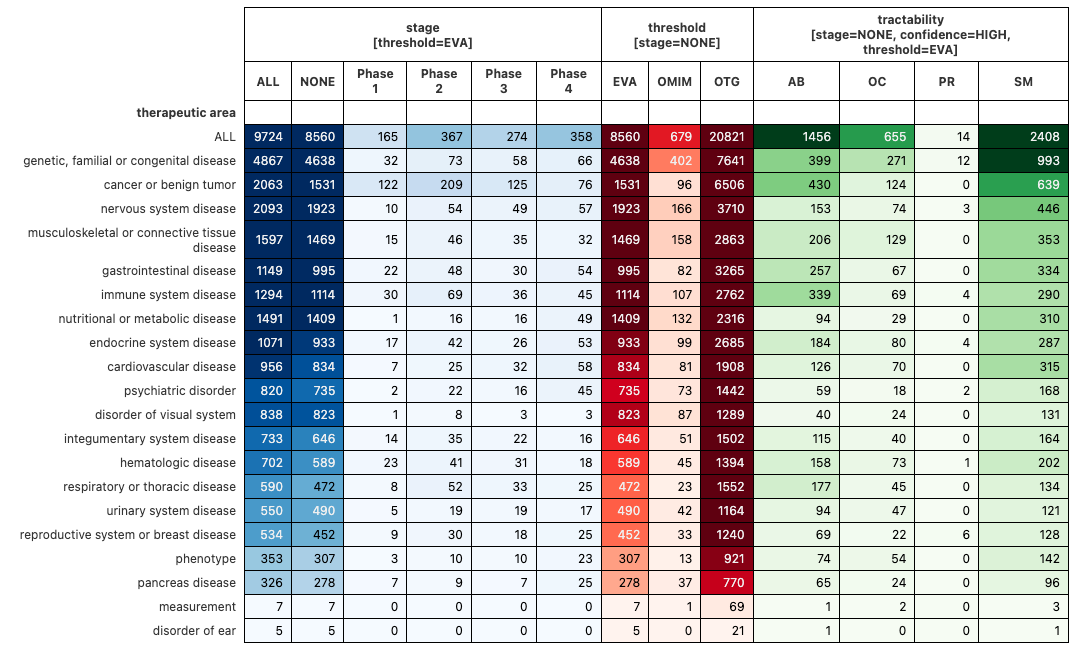
\includegraphics[width=1\textwidth]{opportunity_summary.png}
  \caption{
    \textbf{Present-day target-disease pair counts by stage, likelihood of advancement and tractability}. The \textbf{stage} panel contains counts by maximum trial phase reached, the \textbf{threshold} panel contains counts of pairs with a RDG model score exceeding that of the associated benchmark for only undeveloped pairs, and the \textbf{tractability} panel shows pair frequencies among undeveloped pairs exceeding the EVA threshold that also have a HIGH tractability rating as defined in Supplementary~Table~\ref{tab:tractability_buckets}. This corresponds to targets that have all been in clinical development already, except for the \textbf{OC} modality in which case it indicates that a target has been approved. 
  }
  \label{fig:opportunity_summary}
\end{figure}

Figure~\ref{fig:opportunity_summary} shows the distribution of TD pair counts for select buckets across therapeutic areas as well as across the current maximum phase reached for any one pair. We find that there are $\sim$2,400 small-molecule-enabled, $\sim$1,400 antibody-enabled, and 14 PROTAC-enabled TD pairs with a probability of advancement that is nearly 3x other TD pairs based on the EVA threshold RR=2.93 in Figure~\ref{fig:relative_risk_by_limit}. Top antibody-enabled pairs are shown in Supplementary~Figure~\ref{fig:top_opportunity_predictions} along with their corresponding genetic and clinical support.

We also note that these TD pairs are identified using predictors that are not constrained by temporalization. In other words, the predictions used to identify \textbf{present-day} TD pairs with a high likelihood of clinical success are based on more evidence than what is available in other sections of this study. This is primarily because some evidence in Open Targets is not associated with publications. Ignoring that limitation is appropriate in this context.

\subsection{Inflation}
\label{sec:results_inflation}

Like most studies of this kind, we assume a "closed-world" \cite{Paliwal2020-hr} over the space of target-disease pairs and any evidence between them. This means that we do not differentiate between evidence that an association for any one pair truly does \textbf{not} exist (or is too weak to be relevant under the omnigenic model \cite{PMID:28622505}), and the lack of any attempt to find that evidence in the first place. This also means that our estimate of the prognostic value for any one evidence source is subject to historical trends in biomedical research and the myriad ways that this research can be biased towards particular targets and diseases. We avoid attempting to comprehensively survey these biases in favor of offering an illustrative list of specific examples that are relevant in this study:

\begin{enumerate}
\item Mendelian randomization research is biased towards cardiovascular diseases as they have a disproportionate number of known, modifiable exposures \cite{PMID:36736292}
\item Putative protein interactions that do not result from genome-scale or otherwise unbiased assays result in an overrepresentation of successful drug targets in resources like STRING \cite{PMID:36370105}, thereby inflating the success of network expansion methods over these databases to identify such targets \cite{Sadler2023-xd}.
\item Transcript expression studies run in late-stage clinical trials for a single indication, e.g. \cite{PMID:27723281} linking SLE to IFN genes, are a degenerate indicator of advancement beyond earlier stage trials when the timing of this evidence is not accounted for.
\item Targets tested against more indications in clinical trials enrich for failures because the marginal cost of testing more indications decreases, but the evidence for these indications is often weaker \cite{PMID:33262371}.
\item Herding effects in pharma R\&D pipelines around particular drug targets are becoming increasingly clear over time \cite{PMID:37117303} and generate an excess of clinical evidence for those targets.
\end{enumerate}

We also note that the skew in basic drug target research towards those that already have rich annotations and well characterized molecular function \cite{PMID:29358745} as well as the disproportionate representation of particular target families in pharma R\&D pipelines \cite{PMID:27910877,PPR:PPR7029} and the fact that literature is well known to be biased away from negative results in general \cite{PMID:32893970} are all problematic. 

While it is not possible to address all of these issues, we emphasize that there is a clear pattern across the examples in the list above in that they require \textbf{past} clinical successes and/or failures to arise in the first place. This suggests that accounting for when evidence first emerged would limit the extent of these problems. We do so in this study based solely on publication dates associated with any one piece of information linking target-disease pairs. This also offers a novel opportunity to attempt to quantify what kind of evidence suffers most from these biases. Figure~\ref{fig:evidence_inflation} presents results for this based on a relative risk statistic defined as:

\begin{equation}
  \frac{P(A | B)}{P(A | \neg B)}
\end{equation}

where:

\begin{itemize}
\item \(A\) is the event that evidence for a TD pair arises after its first early-stage (phase 1 or 2) trial rather than before
\item \(B\) is the event that a TD pair advances into late-stage trials (phase 3 or 4)
\end{itemize}

We refer to this as "inflation risk" so as not to confuse it with the relative risk statistic used in all other contexts, and it can be more simply described as the fraction of TD pairs for which evidence arises \textbf{after} the beginning of an ultimately successful early-stage trial divided by that same fraction for TD pairs that do not advance to late-stage trials. The intuition for this statistic is that it will be higher if successful trials lead to the generation of evidence of a particular type, and it should be 1 in cases where the emergence of evidence is independent of clinical success. We also measure this potential lack of independence through the more commonly used Fisher's exact test, e.g. \cite{PMID:19725948}, and both are presented in Figure~\ref{fig:evidence_inflation}.

\begin{figure}[!htb]
  \centering
  \captionsetup{width=.9\linewidth}
  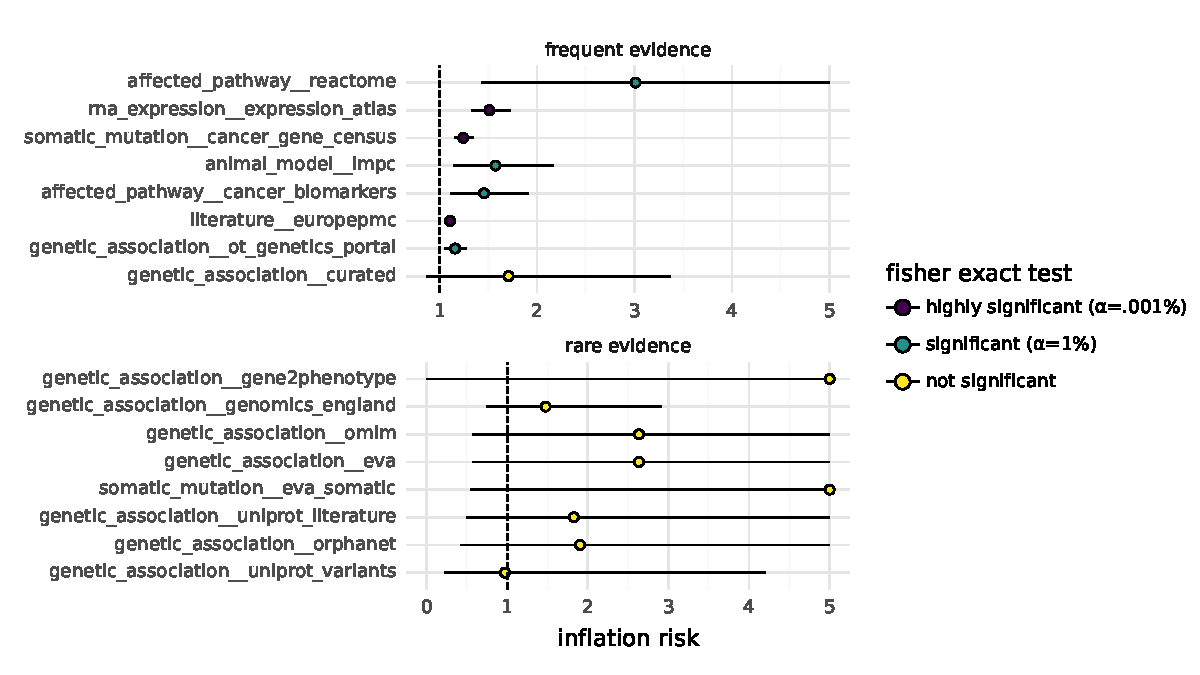
\includegraphics[width=1\textwidth]{evidence_inflation.pdf}
  \caption{
    \textbf{Clinical success drives evidence discovery}.  
  }
  \label{fig:evidence_inflation}
\end{figure}

We find that evidence from Reactome is the worst offender by this metric, implying that it often only arises for TD pairs after a certain level of clinical success has been attained. We also find that long-running aggregators/curators of published research often focused on individual diseases/phenotypes, like Expression Atlas, IMPC, CGS and Cancer Biomarkers exhibit this form of inflation as well.

Sources of genetic evidence appear to be much less inflated, or have too little data to reach significance. This is to be expected for GWAS evidence arising from genome-wide, phenome-wide biobank consortia, however much of historical GWAS evidence is not phenome-wide. More context on how much this is likely to matter comes from \cite{PMID:37612393} in which it was estimated that as few as 6\% of 500 FDA-approved targets for non-cancer drugs arose from programs highly motivated by pre-existing genetic support and that "the remaining 94\% were probably identified using conventional pharmacology, biochemistry or molecular biology approaches". We then speculate that if the initiation of new drug programs was not historically motivated highly by the existence of genetic support, then the incentives for pursing new genetic evidence based on clinical and commercial success are likely to be minimized. This, in conjunction with existing precedent \cite{Nelson2015-eg,King2019-rc,Minikel2023.06.23.23291765,Razuvayevskaya2023.02.07.23285407,PMID:30652614,PMID:35804044} and our inflation results, ultimately led us to the use of genetic evidence without temporalization. In other words, we do not treat genetic evidence as longitudinal features like all others associated with TD pairs. A breakdown of which features are treated in which manner is provided in Table~\ref{tab:features}.

\section{Conclusion}

We have demonstrated that simple machine learning methods applied to longitudinal biomedical evidence from many sources can be used to predict clinical outcomes for combinations of drug targets and diseases, without knowledge of molecular properties or trial design details. We have also shown that these methods are more precise in the extremes of their predictions than composite, heuristic scores like those from Open Targets. They also outperform such baselines by more comprehensive, traditional measures of classifier performance; however, we find this less compelling and easier to accomplish than improving performance among the upper tail of the opportunities implied by the very highest predictions. This framework would also support the addition of new lines of evidence over time well as it is designed to automatically determine the relevance of any new information without intervention.  Lastly, we find that the space of present-day, undeveloped targets within a disease context that both exceed baseline levels of tractability and have a high predicted likelihood of clinical advancement is substantial. It is likely to grow quickly as well since the breadth of much of the underlying evidence is expanding rapidly \cite{PMID:33214558,PMID:36634672,PMID:31491408}.

\section{Discussion}
\label{sec:discussion}

An important question, that remains difficult to answer, is how much target prioritization methods like the one explored in this study can improve the efficiency of drug discovery. One 2018 estimate suggests that improving success rates from phase 1 to approval by 1.4x (from 9.6\% to 13.8\%) would reduce the median R\&D cost for a \textbf{single drug} by \$480 million USD \cite{PMID:32125404}. If a 2x increase in success rates from phase 1 to approval could be expected when pursuing only genetically validated TD pairs \cite{Nelson2015-eg}, then this would increase to a \$686 million cost savings per drug. Pushing that even further to 3x or 4x increase by incorporating more lines evidence, as we have done here, would suggest a per-drug cost savings of \$1.03 billion and \$1.37 billion, respectively. These savings would only be realized for drugs tested against targets and diseases with sufficient supporting evidence, however, we show in Section~\ref{sec:results_opportunities} there are more than 8,000 such opportunities (i.e. untested, present-day TD pairs) where at least a 3x improvement in success rates could be expected.

% TODO: complete this section?
Another way to quantify the impact that employing superior target prioritization strategies could have is to consider what would happen if this was done across the entire pharmaceutical development industry. Our internal research shows that \$130B (92\%) of global pharma R\&D costs (\$150B) are expended on failed assets each year. This assumes an 8\% success rate that if improved by 3x to 24\%, would lead to a total cost savings of approximately \$22B annually ... (WIP)

Throughout the majority of this study, we focus primarily on performance among the top \topRankingPct\% of TD pairs. Reasons for this are introduced in Section~\ref{sec:features} and Section~\ref{sec:metrics}. It is constructive to expand on this choice by comparing it to alternatives, and noting that it is quite likely that many other predictors could improve performance more comprehensively. We offer some evidence of this through the use of a feature indicating how long a TD pair has been in phase 2 trials, which improves wholistic measures of ranking performance like ROC by 12 points (see Figure~\ref{fig:performance_metric_mean_across_ta}) and provides a particularly dramatic lift across the bottom \bottomRankingPct\% of TD pairs. While time is a necessary but not sufficient condition for clinical advancement of a TD pair, given that a single trial can take years to complete, it also correlates with how many distinct trials, drugs, companies, sponsors, investigators, etc. attempt to validate any one pair. We posit that this is crucial because even if a druggable, mechanistic link exists between a target and a disease, many (or even most) trials testing that link will fail (or not even start) for reasons unrelated to efficacy or safety of a drug \cite{Razuvayevskaya2023.02.07.23285407}. Some of these reasons include 1) commercial factors like a lack of funding, pipeline reprioritization and competitive density, 2) administrative or logistical factors like a lack of enrollment, retention problems, poor trial design, drug supply chain shortages, epidemics (COVID-19) and 3) regulatory factors like legislative shifts or extensive regulatory approval delays. Many of these factors are fundamentally difficult or impossible to predict. Epidemic outbreaks, labor shortages leading to supply chain problems and regulatory shifts are examples of exogenous shocks for which accurate predictors are unlikely to exist. However, factors like funding, competition, enrollment and certain aspects of trial design have measurable predictors such as preceding venture capital and private equity investments, patent filings and revenue for related drugs, disease severity and prevalence, and the existence of biomarkers or other enabling factors for better trial designs (respectively). As a more detailed example, patient recruitment failures are the most common reason trials fail \cite{Razuvayevskaya2023.02.07.23285407} and recruitment statistics are highly predictive of eventual trial outcomes \cite{Lo2019Machine,PMID:34430930}. It stands to reason then that predicting trial enrollment failures well in advance of when a trial is even conceived, i.e. for a target-disease pair, should be possible because recruitment in trials is determined, in part, by how prevalent a disease is, how debilitating it is, what patient demographics it inflicts, whether existing treatments exist for it and how successful recruitment for past trials has been -- all of which are measurable. Signals like this could be used to further improve performance since they better capture causal factors in non-biological advancement failures that time under development -- the only non-biological feature in this study -- does not.

Another notable focus of this study is on evidence for TD pairs that can be \textbf{directly} attributed to them. This is a departure from earlier research in this space like \cite{Nelson2015-eg} that often includes measures of similarity between disease ontology terms to account for the fact that bridging disease nomenclatures used in clinical trial datasets with those used in databases maintaining genetic evidence is difficult. It is not uncommon for disease terms from either source to be sufficiently similar such that it is appropriate to consider them as equivalent. It can also be argued that similarity between disease terms offers an important dimension for expanding evidence in a biologically meaningful way, regardless of technical mapping issues. This is taken to further extremes in studies like \cite{PMID:33262371} that propagates evidence using both measures of target similarity (e.g. using protein interaction networks) and measures of disease similarity (e.g. using ontologies and literature co-occurrence). We believe such expansion methods are very compatible with our approach by either using them to derive new predictors or to propagate predictions from models like these across networks or knowledge graphs.

All results we have presented are based on quasi-prospective outcomes. As described in Section~\ref{sec:introduction}, this means that the outcomes are not truly observed in the future relative to the information used to predict them. Both outcomes and predictors are assigned timestamps corresponding to publication or database dates that approximately capture when the events associated with them actually occurred. The accuracy of that approximation is difficult to determine, and publication dates can be particularly inaccurate when they lag evidence discovery by months or years. This does not pose a risk for information leaks in a quasi-prospective formulation though, as long as the date associated with an event does not precede its occurrence. Nevertheless, it is possible that publication dates are simply entered into a database incorrectly, clinical trial registries inaccurately represent when trials began or ended, or that information from future events ends up associated with the wrong targets and/or diseases. These are only a few possible risks for information leaks, and though each is relatively rare on its own, their combined impact could be substantial. And as with all forecasting models, the accuracy of future predictions is reliant on the extent to which the underlying data generating process may either change or deviate from anticipated changes. Fortunately, the evidence we employ as predictors here comes predominantly from molecular interactions in humans, animals or cells that are likely to remain stable in time, or shift on evolutionary time scales that eclipse drug development timelines. This summary on the subject from \cite{PMID:33262371} is pertinent:

\begin{quotation}
  It is important to bear in mind therefore that what we are measuring when looking at historical trial outcomes is not an unbiased measure of any given gene's true disease associations, but rather a view on how useful a given evidence source or analytical method has been for choosing drug targets based on current and historical drug discovery practices. Dramatic changes in these practices in the future could render some of our conclusions obsolete, though the fundamental observation that genetic association itself is retained in molecular networks will remain valid.
\end{quotation}

Model performance evaluations based on prospective outcomes, as an alternative to quasi-prospective outcomes, offer a number of distinct advantages. For one, they mitigate nearly all the risks for information leaks mentioned previously by ensuring that all predictive information precedes clinical outcomes. They also offer a means to quantify those risks. An extension of this work might utilize the Open Targets database snapshots, dating back as far as 2016, to examine how much model performance differs between models trained on features from a snapshot and models trained on data from a current Open Targets release with features that are temporalized and then filtered to not exceed the year of the earlier snapshot. Similarly, that extension could examine how much model performance differs for a snapshot with and without longitudinal features by considering only outcomes that occurred after the snapshot. Such an approach could also be applied on a per-feature basis to gain more granular insight on which kinds of evidence pose the greatest risk. One clear disadvantage of prospective evaluation for this problem is that it requires years to accrue enough future clinical outcomes to be meaningful. This also means that predictors must omit that many years of accrued evidence as well, which can deflate performance compared to what is possible in the present day. Another disadvantage is that it is significantly more difficult to operationalize prospective evaluations, thereby implying that the decrease in risk of information leaks may be partially offset by an increase in technical risk.

\section{Methods}
\label{sec:methods}

All data used in this study comes from Open Targets with one minor exception. Open Targets provides PubMed identifiers as provenance for evidence without supplying publication dates or years in all cases. These dates are taken from \cite{PMID:33763309} instead. Our primary results are based on the 23.12 Open Targets release, but we also use releases 23.09 and 23.06 as part of our sensitivity analysis in section \ref{sec:sensitivity}. 

The features we derive from Open Targets come primarily from a single target-disease dataset containing only "direct" evidence \cite{OTdirectVsIndirect}. These features are named according to the \colorbox{Gainsboro}{datasourceId} field within this dataset, and the values for those features are defined as the cumulative, maximum score observed when ordering those scores by the years associated with the evidence underlying them. We also add 2 genetic features that are not immediately available. The first, \colorbox{Gainsboro}{genetic\_association\_\_curated} is a union of all genetic association sources other than \colorbox{Gainsboro}{gene\_burden} and \colorbox{Gainsboro}{ot\_genetics\_portal}. The second, \colorbox{Gainsboro}{genetic\_association\_\_omim}, is defined as any EVA associations with a publication date.

The target-specific features we derive come from the "target prioritisation" dataset \cite{OTtargetPrioritisation}. The only exception to this is a feature defining the maximum trial phase reached, which comes from the primary target-disease evidence dataset. Most scores in this dataset were not used because they cannot be temporalized. We make exceptions for those arising from large-scale, genome-wide assays like LOEUF from gnomAD \cite{PMID:32461654} and tissue expression scores from Human Protein Atlas \cite{PMID:25613900}. We retain a score derived from phenotype severity observed in mice knock-outs \cite{PMID:33231642} as well. All three of these feature sources are unique in that they are imputed differently from all other features when absent in model training. The "closed-world" assumption discussed in Section~\ref{sec:results_inflation} implies that a constant, zero imputation for most missing features is appropriate. This is not true for non-clinical, target-specific fields -- they are mean-imputed instead.

All ridge regression models (e.g. RDG) are fit using the scikit-learn \colorbox{Gainsboro}{Ridge} implementation and all gradient-boosted machine models (e.g. GBM-T) are fit using the LightGBM \cite{LightGBM} algorithm. Ridge models are fit with very weak regularization (\colorbox{Gainsboro}{alpha=1e-6}) and LightGBM models are fit with default settings. Variants of both models are fit, in some cases, with non-negative monotonicity constraints. An important caveat unique to our use of the ridge regression models is that when report results for feature ablations, as in Section~\ref{sec:model_comparison}, all features are actually used to train the models before using only the unablated features to make predictions.

Most results reported in this study consider only a subset of therapeutic areas within the Experimental Factor Ontology (EFO) \cite{PMID:20200009}. All therapeutic areas are retained if they possessed at least 100 TD pairs with target-disease-specific evidence of any kind within our evaluation dataset. We also explicitly omit the "biological\_process", "pregnancy or perinatal disease", "injury, poisoning or other complication", "pregnancy or perinatal disease", "medical procedure", "infectious disease", and "animal disease" therapeutic areas, as they are either not relevant or poorly represented. The "infectious disease" therapeutic area is a borderline case that we omit not because it is necessarily irrelevant, but because it has only 115 associated TD pairs. This makes it the most poorly represented therapeutic area that is possibly relevant. We remove it by explicit omission and use a 100 TD pair threshold rather than using a 115 TD pair threshold.

\section{Limitations}

There are a number of limitations and caveats with this study. These include:

\begin{enumerate}
  \item Open Targets does not currently provide drug approvals with associated dates. This is a part of the reason why we have chosen to focus only on advancement beyond phase 2, and not phase 3 as well. 
  \item Not all Open Targets evidence can be associated with publication dates. This evidence is ignored when used to construct longitudinal predictors; however, this limitation does not apply to Section~\ref{sec:results_opportunities}.
  \item The Open Targets composite score we use (OTS) is not equivalent to the overall composite score for TD pairs provided by Open Targets \cite{OTscoring}. The score they provide is not longitudinal. We create an approximation of it over time based on the same weighting scheme across evidence types, but without a harmonic sum aggregation function. Maximum scores for the same target, disease, year and evidence type combination are used instead.
  \item Estimating an absolute number of TD pairs associated with any criteria is difficult. In Section~\ref{sec:results_opportunities}, we present absolute counts of undeveloped TD pairs with tractable targets and a high likelihood of clinical success. These counts may be inflated by the fact that the associated targets and diseases are so sufficiently similar that they ought not to be counted as distinct examples. Defining a threshold for similarity to combat this problem is difficult and application-specific though, so we do not offer any solutions here.
  \item The source of OMIM associations we use is derived from a subset of associations available in EVA. This subset is defined by associations with a linked publication. This is only an approximation, but our internal research shows that 98\% of EVA records with linked publications also have at least one OMIM submission.
\end{enumerate}

\pagebreak

\section{Appendix}

\begin{figure}[H]
  \centering
  \captionsetup{width=.9\linewidth}
  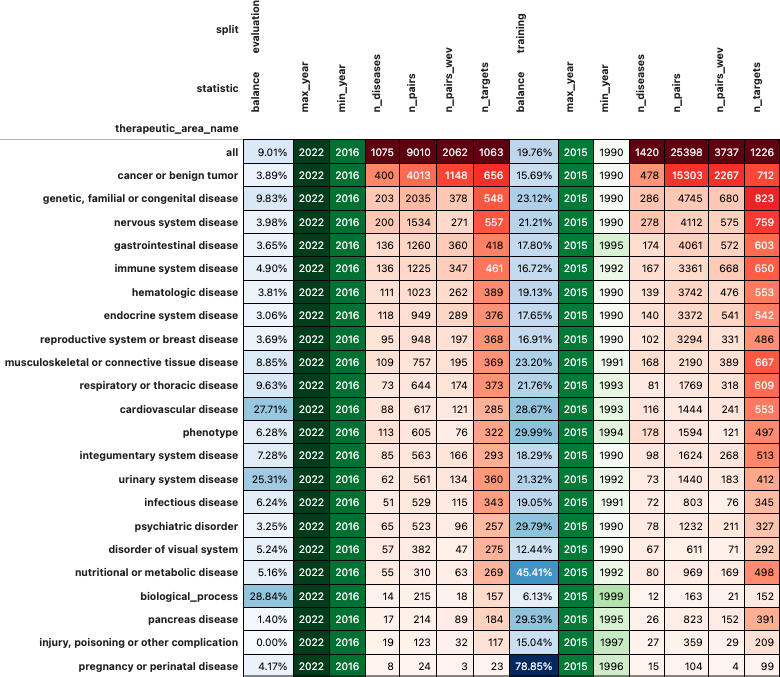
\includegraphics[width=1\textwidth]{dataset_statistics.png}
  \caption{
    \textbf{Training and evaluation dataset summary statistics}.\\\hspace{\textwidth}
    \textbf{balance}: percentage of TD pairs that eventually advanced beyond phase 2 \\\hspace{\textwidth} 
    \textbf{min\_year}: earliest year in which a TD pair has first advanced to phase 2 \\\hspace{\textwidth} 
    \textbf{n\_targets}: number of unique targets \\\hspace{\textwidth} 
    \textbf{n\_diseases}: number of unique diseases \\\hspace{\textwidth} 
    \textbf{n\_pairs}: number of TD pairs (equal to number of records) \\\hspace{\textwidth} 
    \textbf{n\_pairs\_wev}: number of TD pairs with directly associated evidence (i.e. not just target or disease evidence).
  }
  \label{fig:dataset_statistics}
\end{figure}

\pagebreak

\begin{table}
\centering
\caption{Features used in modeling and analysis}
\label{tab:features}
\begin{tabular}{llll}
\toprule
 & feature & entity & kind \\
\midrule
1 & disease\_\_clinical\_\_phase\_max\_\_reached & disease & temporal \\
2 & target\_\_clinical\_\_phase\_max\_\_reached & target & temporal \\
3 & target\_\_genetic\_constraint & target & static \\
4 & target\_\_mouse\_ko\_score & target & static \\
5 & target\_\_tissue\_distribution & target & static \\
6 & target\_\_tissue\_specificity & target & static \\
7 & target\_disease\_\_affected\_pathway\_\_cancer\_biomarkers & target\_disease & temporal \\
8 & target\_disease\_\_affected\_pathway\_\_crispr & target\_disease & temporal \\
9 & target\_disease\_\_affected\_pathway\_\_crispr\_screen & target\_disease & temporal \\
10 & target\_disease\_\_affected\_pathway\_\_progeny & target\_disease & temporal \\
11 & target\_disease\_\_affected\_pathway\_\_reactome & target\_disease & temporal \\
12 & target\_disease\_\_affected\_pathway\_\_slapenrich & target\_disease & temporal \\
13 & target\_disease\_\_affected\_pathway\_\_sysbio & target\_disease & temporal \\
14 & target\_disease\_\_animal\_model\_\_impc & target\_disease & temporal \\
15 & target\_disease\_\_genetic\_association\_\_clingen & target\_disease & static \\
16 & target\_disease\_\_genetic\_association\_\_curated & target\_disease & static \\
17 & target\_disease\_\_genetic\_association\_\_eva & target\_disease & static \\
18 & target\_disease\_\_genetic\_association\_\_gene2phenotype & target\_disease & static \\
19 & target\_disease\_\_genetic\_association\_\_gene\_burden & target\_disease & static \\
20 & target\_disease\_\_genetic\_association\_\_genomics\_england & target\_disease & static \\
21 & target\_disease\_\_genetic\_association\_\_omim & target\_disease & static \\
22 & target\_disease\_\_genetic\_association\_\_orphanet & target\_disease & static \\
23 & target\_disease\_\_genetic\_association\_\_ot\_genetics\_portal & target\_disease & static \\
24 & target\_disease\_\_genetic\_association\_\_uniprot\_literature & target\_disease & static \\
25 & target\_disease\_\_genetic\_association\_\_uniprot\_variants & target\_disease & static \\
26 & target\_disease\_\_known\_drug\_\_chembl & target\_disease & temporal \\
27 & target\_disease\_\_literature\_\_europepmc & target\_disease & temporal \\
28 & target\_disease\_\_outcome\_\_advanced & target\_disease & temporal \\
29 & target\_disease\_\_rna\_expression\_\_expression\_atlas & target\_disease & temporal \\
30 & target\_disease\_\_somatic\_mutation\_\_cancer\_gene\_census & target\_disease & temporal \\
31 & target\_disease\_\_somatic\_mutation\_\_eva\_somatic & target\_disease & temporal \\
32 & target\_disease\_\_somatic\_mutation\_\_intogen & target\_disease & temporal \\
33 & target\_disease\_\_time\_\_transition & target\_disease & temporal \\
\bottomrule
\end{tabular}
\end{table}


\clearpage

\section{Supplementary Material}

\pagebreak

\begin{figure}[H]
  \centering
  \captionsetup{width=.9\linewidth}
  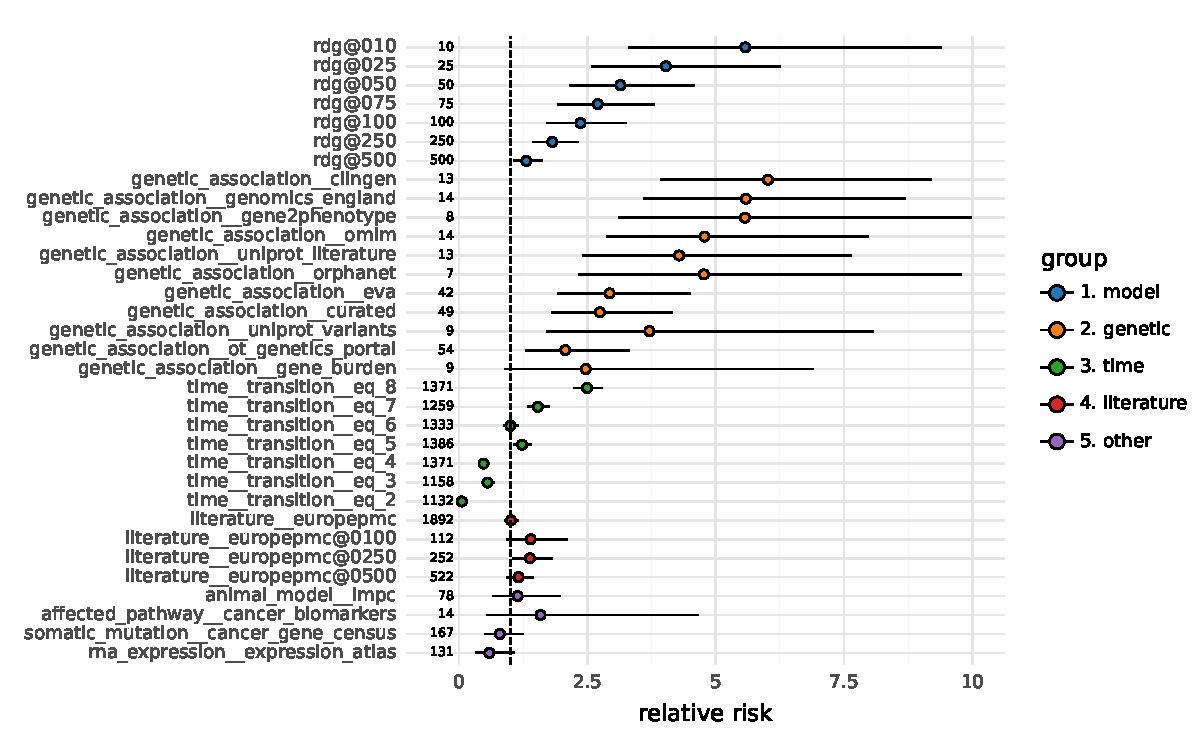
\includegraphics[width=1\textwidth]{relative_risk_core_features.pdf}
  \caption{
    \textbf{Performance of individual features and predictive scores as measured by relative risk}.
    RDG model results denoted by \colorbox{Gainsboro}{rdg@N} indicate performance for the \colorbox{Gainsboro}{N} top TD pairs. The same convention is used for \colorbox{Gainsboro}{literature} evidence and the \colorbox{Gainsboro}{time\_\_transition\_\_eq\_X} convention denotes RR estimates when the time since the phase 2 transition is equal to \colorbox{Gainsboro}{X} years. The \colorbox{Gainsboro}{omim}, \colorbox{Gainsboro}{eva}, and \colorbox{Gainsboro}{ot\_genetics\_portal} features correspond to the OMIM, EVA and OTG baselines of Figure~\ref{fig:relative_risk_by_limit}, respectively. All other features are assessed based on their existence. The counts along the origin indicate how many TD pairs were used to compute the RR numerator.
  }
  \label{fig:relative_risk_core_features}
\end{figure}

\pagebreak

\begin{figure}[H]
  \centering
  \captionsetup{width=.9\linewidth}
  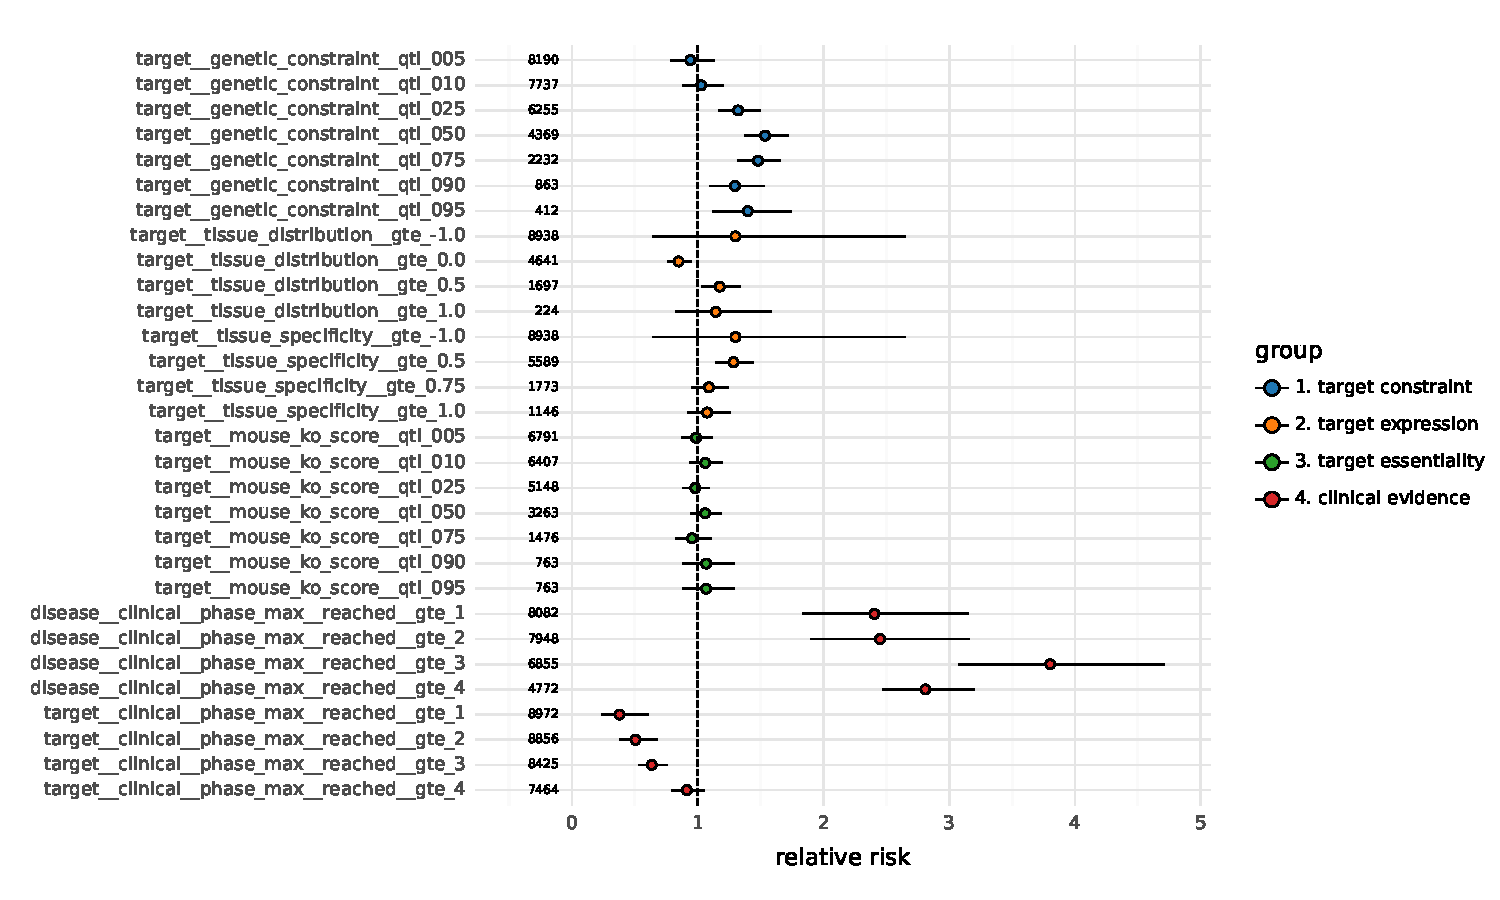
\includegraphics[width=1\textwidth]{relative_risk_static_features.pdf}
  \caption{
    \textbf{Relative risk scores for target/disease features}.
    The features ending with \colorbox{Gainsboro}{qtl\_Q} denote binary indicators constructed from cases where the feature meets or exceeds quantile \colorbox{Gainsboro}{Q} of its distribution. The features ending with \colorbox{Gainsboro}{gte\_X} denote indicators for when the feature meets or exceeds a specific value \colorbox{Gainsboro}{X}.
  }
  \label{fig:relative_risk_static_features}
\end{figure}

\pagebreak

\begin{figure}[H]
  \centering
  \captionsetup{width=.9\linewidth}
  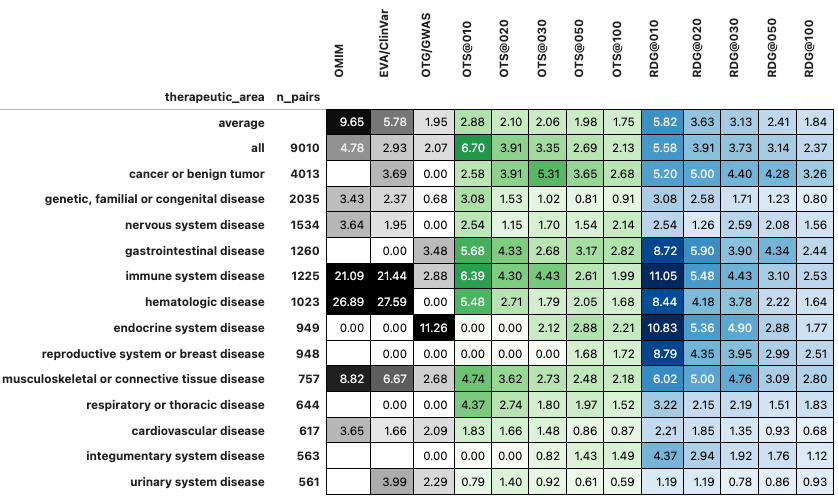
\includegraphics[width=1\textwidth]{relative_risk_by_ta.png}
  \caption{
    \textbf{Relative risk scores by method, benchmark and therapeutic area}.
    The \textbf{average} therapeutic area indicates mean values across all others except for \textbf{all}, which is an ungrouped estimate across all diseases regardless of therapeutic area.
  }
  \label{fig:relative_risk_by_ta}
\end{figure}
  
\pagebreak

\begin{figure}[H]
  \centering
  \captionsetup{width=.9\linewidth}
  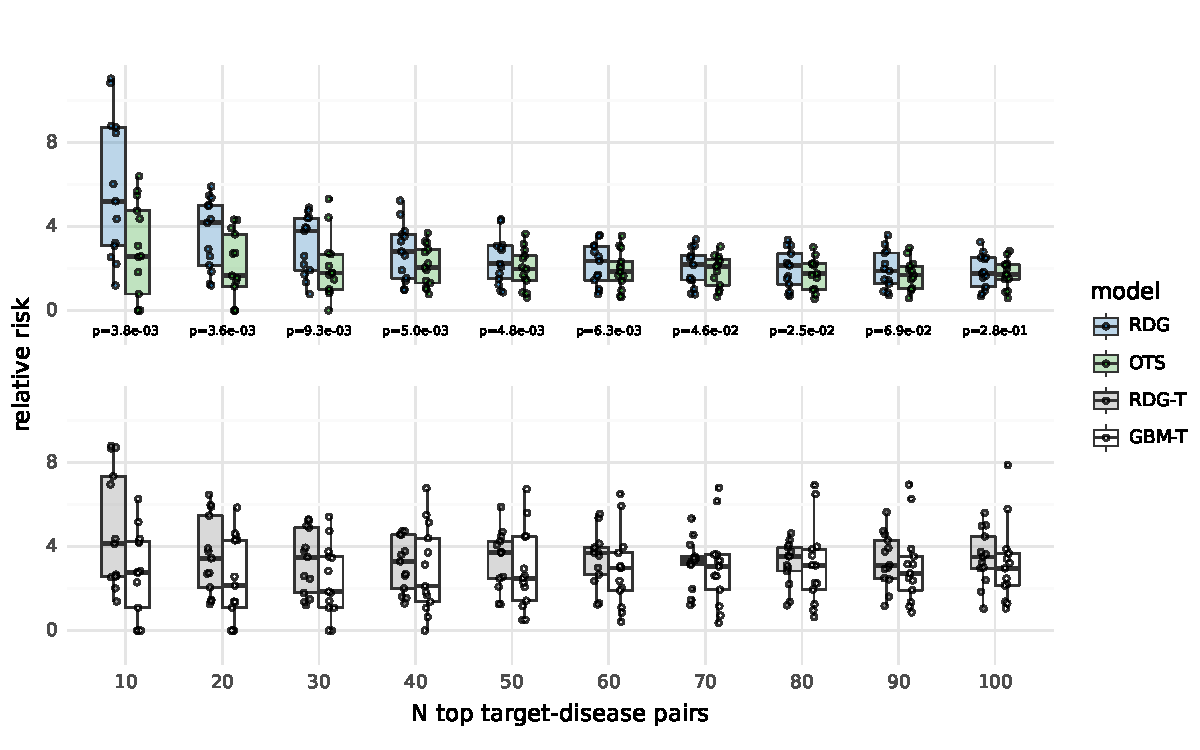
\includegraphics[width=1\textwidth]{relative_risk_dist_across_ta.pdf}
  \caption{
    \textbf{Relative risk distributions across select therapeutic areas}.
    P-values are computed from a one-sided Wilcoxon signed-rank test with the alternative that the RDG model RR averages across therapeutic areas exceed OTS averages.
  }
  \label{fig:relative_risk_dist_across_ta}
\end{figure}

\pagebreak

\begin{figure}[H]
  \centering
  \captionsetup{width=.9\linewidth}
  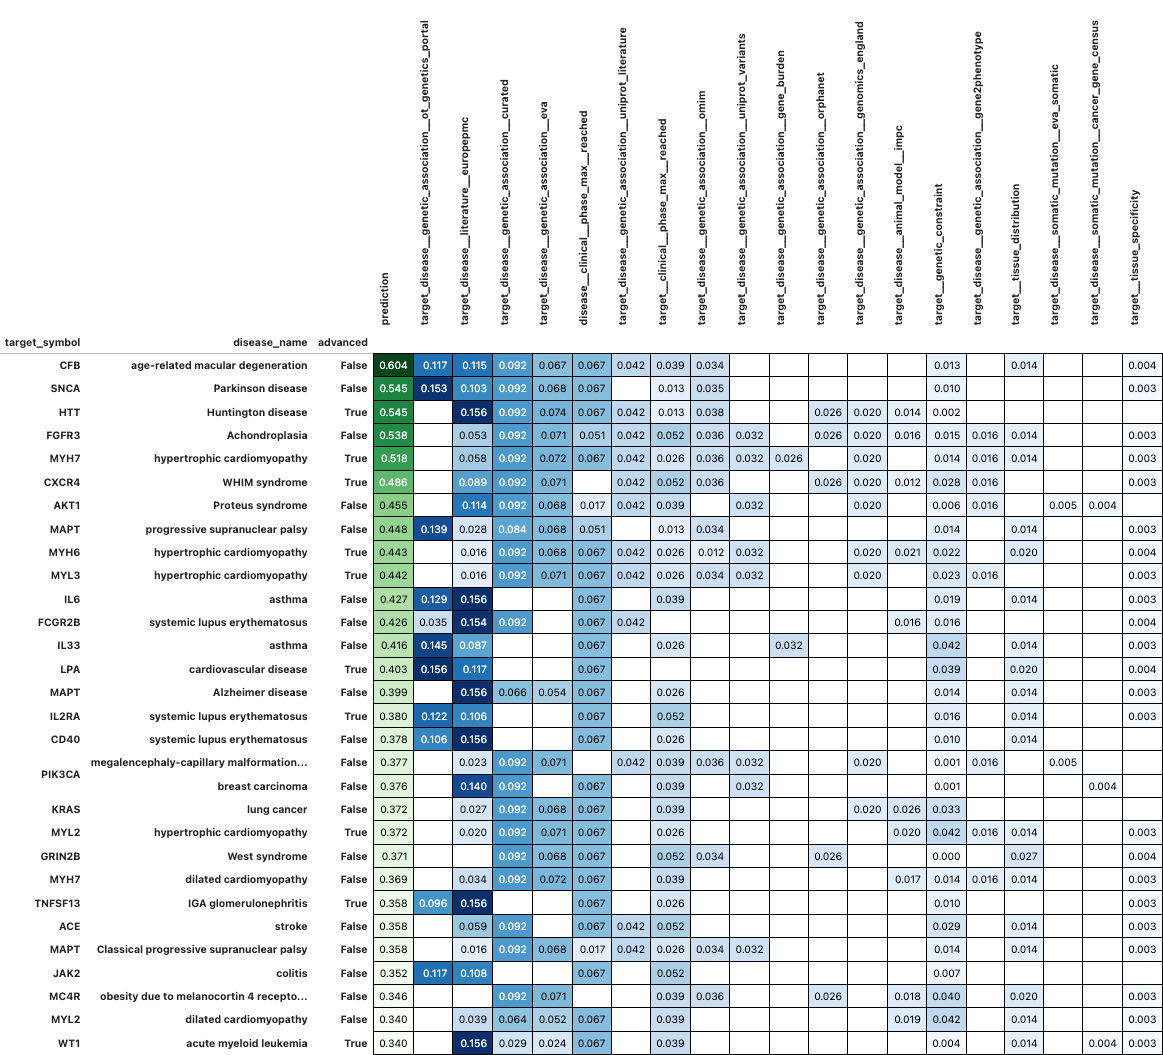
\includegraphics[width=1\textwidth]{top_evaluation_predictions.png}
  \caption{
    \textbf{Top RDG model evaluation dataset predictions}.
    Feature contributions are shown as the product of their underlying values and the RDG coefficients. The \textbf{advanced} field indicates whether the associated TD pair advanced beyond phase 2 as of 2024.
  }
  \label{fig:top_evaluation_predictions}
\end{figure}


\pagebreak

\begin{table}
\centering
\caption{Tractability bucket assignments}
\label{tab:tractability_buckets}
\begin{tabular}{llll}
\toprule
 & evidence & modality & confidence \\
\midrule
1 & Phase 1 Clinical & OC & LOW \\
2 & Advanced Clinical & OC & MED \\
3 & Approved Drug & OC & HIGH \\
4 & GO CC med conf & AB & LOW \\
5 & Human Protein Atlas loc & AB & LOW \\
6 & UniProt SigP or TMHMM & AB & LOW \\
7 & UniProt loc med conf & AB & LOW \\
8 & GO CC high conf & AB & MED \\
9 & UniProt loc high conf & AB & MED \\
10 & Advanced Clinical & AB & HIGH \\
11 & Approved Drug & AB & HIGH \\
12 & Phase 1 Clinical & AB & HIGH \\
13 & Database Ubiquitination & PR & LOW \\
14 & Half-life Data & PR & LOW \\
15 & Small Molecule Binder & PR & LOW \\
16 & Literature & PR & MED \\
17 & UniProt Ubiquitination & PR & MED \\
18 & Advanced Clinical & PR & HIGH \\
19 & Phase 1 Clinical & PR & HIGH \\
20 & Druggable Family & SM & LOW \\
21 & High-Quality Pocket & SM & LOW \\
22 & Med-Quality Pocket & SM & LOW \\
23 & High-Quality Ligand & SM & MED \\
24 & Structure with Ligand & SM & MED \\
25 & Advanced Clinical & SM & HIGH \\
26 & Approved Drug & SM & HIGH \\
27 & Phase 1 Clinical & SM & HIGH \\
\bottomrule
\end{tabular}
\end{table}


\clearpage

\begin{figure}[H]
  \centering
  \captionsetup{width=.9\linewidth}
  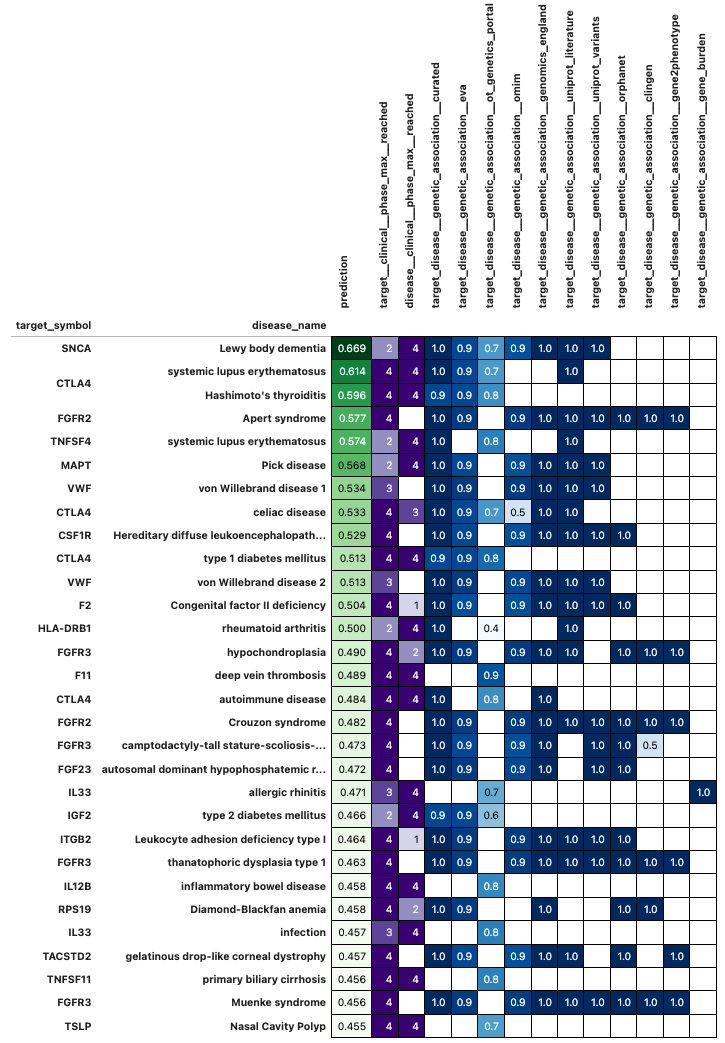
\includegraphics[width=.9\textwidth]{top_opportunity_predictions.png}
  \caption{
    \textbf{Top ranked undeveloped, tractable target-disease pairs}. The highest scoring TD pairs per the RDG model that have not entered clinical trials despite having a target that has been in trials of an antibody-based drug. All values shown other than \textbf{prediction} are raw feature values, unweighted by RDG coefficients.
  }
  \label{fig:top_opportunity_predictions}
\end{figure}

\pagebreak

\subsection{Sensitivity}
\label{sec:sensitivity}

In order to validate the stability of our findings in Section~\ref{sec:results_performance}, we repeat this analysis across 18 different configurations listed in Supplementary~Table~\ref{tab:sensitivity_configurations}. This includes 3 separate versions of Open Targets, 3 choices for the year defining the split between training and evaluation data and 2 choices for the length of the minimum advancement window (in years).

We find that the mean RR values from the RDG model consistently exceed the OTS model in all configurations among the very highest rankings (N=10) and also exceed the OTS model in all configurations except for 1 for N between 20 and 60. This data is shown in Supplementary~Figure~\ref{fig:sensitivity_relative_risk}. The significance of these differences drops notably after N=40, which can be seen in the distribution of p-values from a Wilcoxon signed-rank test shown in Supplementary~Figure~\ref{fig:sensitivity_p_values}.

\begin{table}
\centering
\caption{Configurations for sensitivity analysis}
\label{tab:sensitivity_configurations}
\begin{tabular}{llrr}
\toprule
 & open\_targets\_version & max\_training\_year & min\_time\_to\_advancement\_years \\
\midrule
1 & 23.09 & 2017 & 4 \\
2 & 23.12 & 2017 & 2 \\
3 & 23.09 & 2015 & 2 \\
4 & 23.12 & 2015 & 2 \\
5 & 23.09 & 2017 & 2 \\
6 & 23.06 & 2015 & 4 \\
7 & 23.06 & 2017 & 2 \\
8 & 23.06 & 2013 & 2 \\
9 & 23.06 & 2015 & 2 \\
10 & 23.06 & 2017 & 4 \\
11 & 23.12 & 2013 & 4 \\
12 & 23.09 & 2015 & 4 \\
13 & 23.09 & 2013 & 2 \\
14 & 23.12 & 2013 & 2 \\
15 & 23.09 & 2013 & 4 \\
16 & 23.12 & 2017 & 4 \\
17 & 23.12 & 2015 & 4 \\
18 & 23.06 & 2013 & 4 \\
\bottomrule
\end{tabular}
\end{table}


\clearpage

\begin{figure}[H]
  \centering
  \captionsetup{width=.9\linewidth}
  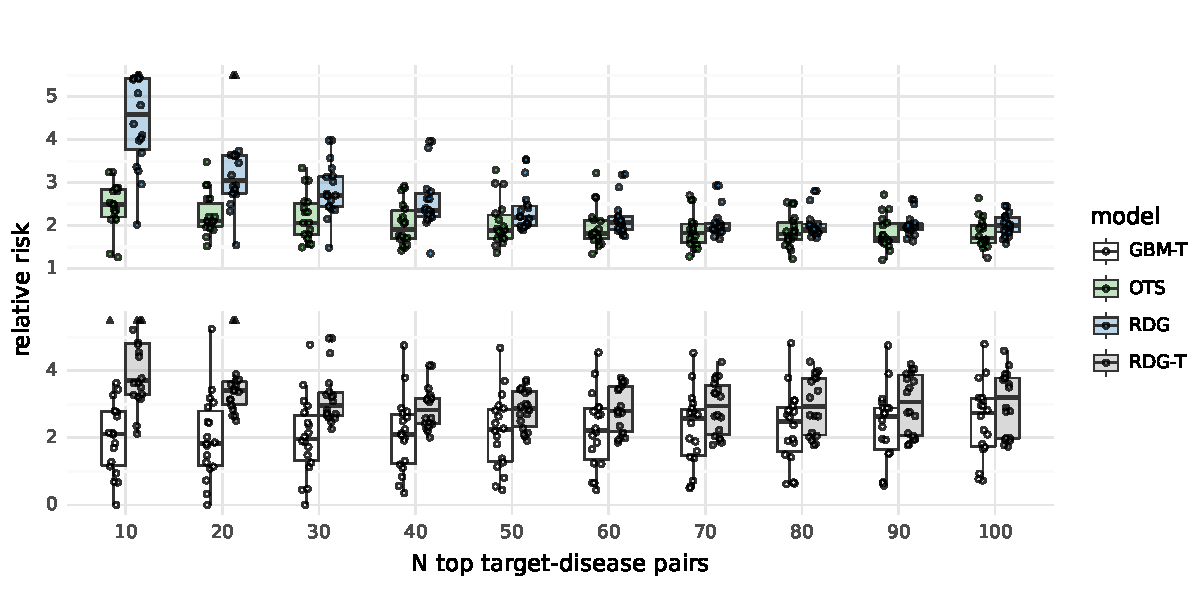
\includegraphics[width=1\textwidth]{sensitivity_relative_risk.pdf}
  \caption{
    \textbf{Relative risk distributions across configurations in sensitivity analysis}.
    The distribution of the mean RR values displayed for a single configuration in Figure~\ref{fig:performance_across_ta} is shown here across 18 configurations.
  }
  \label{fig:sensitivity_relative_risk}
\end{figure}

\pagebreak

\begin{figure}[H]
  \centering
  \captionsetup{width=.9\linewidth}
  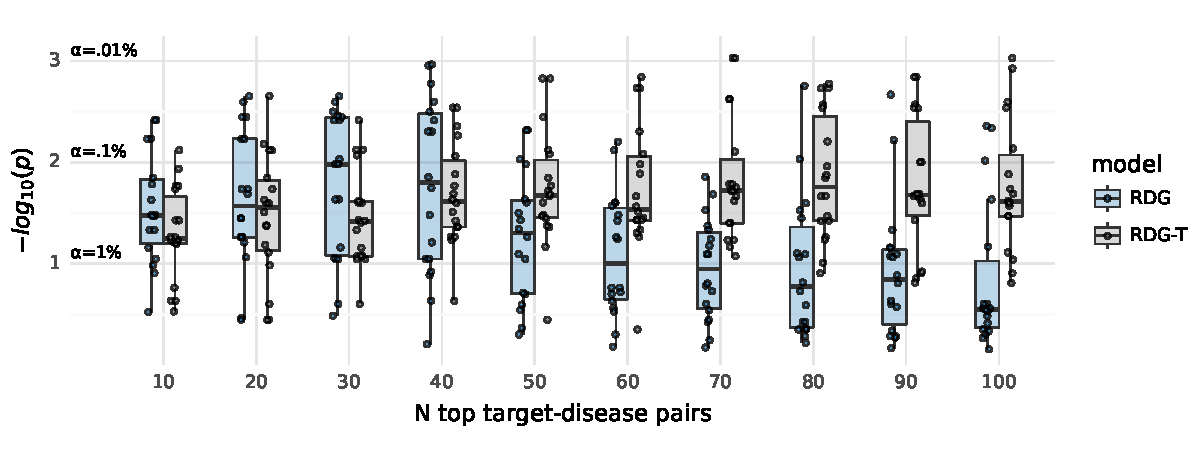
\includegraphics[width=1\textwidth]{sensitivity_p_values.pdf}
  \caption{
    \textbf{P-value distributions across configurations in sensitivity analysis}.
    The distribution of the p-values displayed for a single configuration in Supplementary~Figure~\ref{fig:relative_risk_dist_across_ta} is shown here across 18 configurations.
  }
  \label{fig:sensitivity_p_values}
\end{figure}

\pagebreak

\bibliographystyle{unsrt}  
\bibliography{references} 

\end{document}
